\documentclass{article}

\usepackage{hyperref}
\hypersetup{
	colorlinks=true,
	linkcolor=blue,
	filecolor=magenta,      
	urlcolor=cyan
}
\usepackage[american]{circuitikz}
\usepackage{siunitx}
\usepackage{amsmath}

\begin{document}
	\section{Working of a Regular Current Mirror}
		\href{https://www.youtube.com/watch?v=x9xt9ChSiow&ab_channel=ALLABOUTELECTRONICS}{Useful Youtube Video}
		\begin{center}
			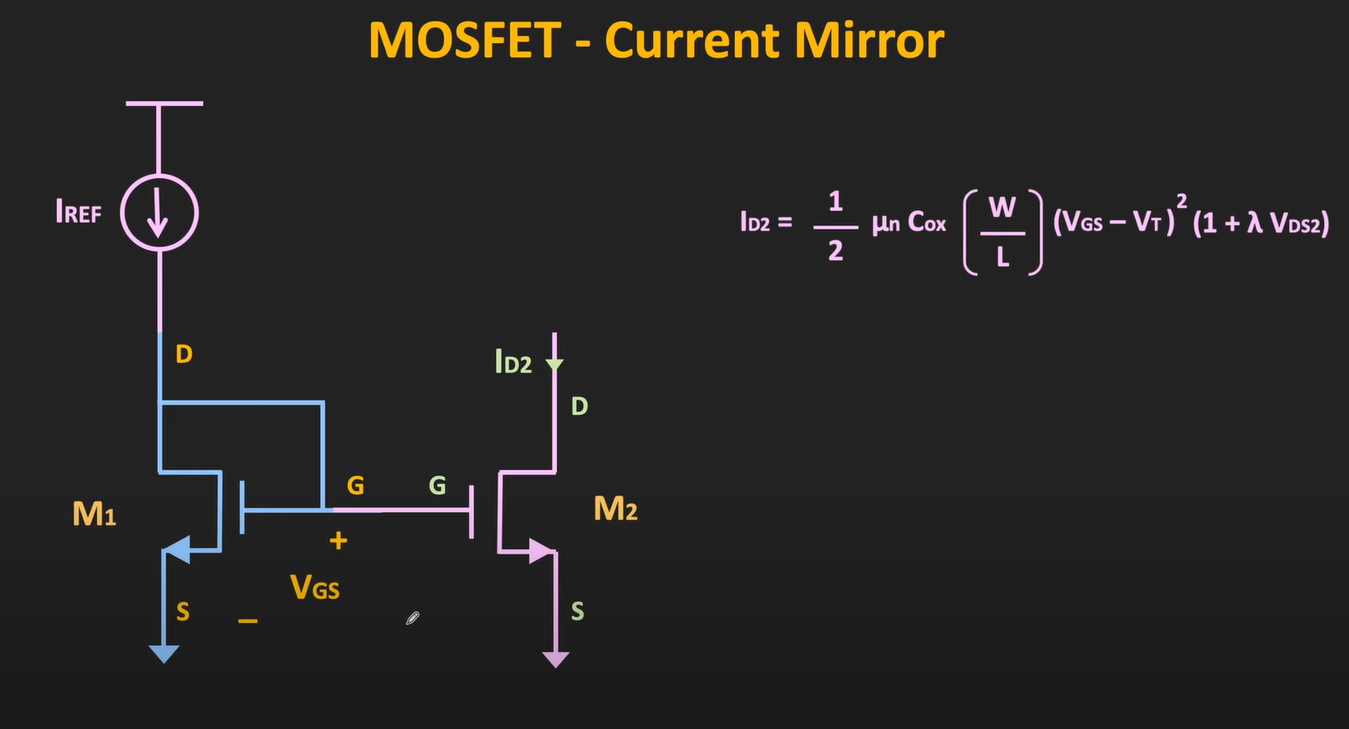
\includegraphics[width=\textwidth]{imgs/screenshot1.png}
		\end{center}
		I want to point out that the regular current mirror, M1 is diode connected so it always stays in saturation. Its drain current equation without channel length modulation ($\lambda=0$) is
		\begin{align*}
			V_G&=V_D\\
			I_{D1}&=\frac{1}{2}\mu_n C_{ox}\left(W/L\right)(V_{DS}-V_t)^2
		\end{align*}
		We see that the free variables are $I_{D1}$ and $V_{DS}$, current source $I_{REF}$ is used to set $I_{D1}$, which sets $V_{DS}$, which sets $V_G$. On the other side, M2's drain current ($\lambda=0$) is 
		\begin{align*}
			I_{D2}&=\frac{1}{2}\mu_n C_{ox}\left(W/L\right)(V_{GS}-V_t)^2
		\end{align*}
		The only moving variable is $V_{GS}$. This is saying that $I_{D2}$ can be set by $V_G$ only, and M2's drain current doesn't depend on $V_{DS}$ of M2!!\\
		However this is no longer true once channel length modulation is introduced. $\lambda$ brings a small deviation when setting $I_{D2}$ to be our $I_{REF}$, but it's still pretty close.
\end{document}